% SJK: Document template originally from Andy Maloney "untitled.tex"
\documentclass{article}

%	Packages used.
\usepackage{amsmath}
\usepackage{fullpage}
\usepackage{graphicx}
\usepackage{caption}
\usepackage{subcaption}
%% see: http://en.wikibooks.org/wiki/LaTeX/Floats,_Figures_and_Captions#Subfloats

\begin{document}
	\section{Summary of 4.1 Guassian mixture models}

	\begin{itemize}
		\item The first example generates random data with a mixture of gaussians at two different points.  It's pretty simple, and most of my confusion comes from numpy and array shaping / concatenating things.  See Figure \ref{fig:GMMex} for examples with a few different number of components for model.
		\item Next, I followed the Gaussian Mixture Model (GMM), using the Expectation-Minimization (EM) method on the iris data set (using all 4 dimensions, showing only two of those dimensions.  I was confused by the method at first, because it seemed supervised, and then I realized it is partially supervised.  The code for testing the four different covariance constraints, along with making the ellipses is quite complicated.  I learned a lot, but still wouldn't be comfortable writing that from scratch.  Maybe I'll never have to, because there are so many examples to work from. See Figure \ref{fig:GMM_orig} for replication of the tutorial.
		\item For fun, I attempted to use the DPGMM model on the iris dataset.  This sort of prooved the above point, that it's very easy to adapt the example code.  Although, for many different alpha choices, nothing could come close.  This is either because I'm using DPGMM incorrectly, or, I think more likely, because unsupervised DPGMM will never work on the iris data set.  See Figure \ref{fig:GMMfail} for the plot of failed attempt.
		\item For almost all of the work up to now, I've been typing the python code in by hand, as it really helps with learning.  For now, though, I cut and pasted to do the GMM selection based on BIC (Baysian Information Criterion) example.  There really isn't too much new stuff, except a whole lot of plotting.  It's still just using a bunch of GMM models and then extracting the BIC score from the model. I then switched from BIC to AIC (file plot\_gmm\_selection2.py), and I cannot graphically discern any difference (bummer).  See Figure \ref{fig:GMMSelectOrig} for BIC example. I decreased the number of data points to 15 (from 600), got rid of the random number seed, and then sometimes I got other models to win.  See Figure \ref{fig:GMMSelect15}
	\end{itemize}

    \begin{figure}
            \centering
            \begin{subfigure}[h]{0.3\textwidth}
                    \centering
                    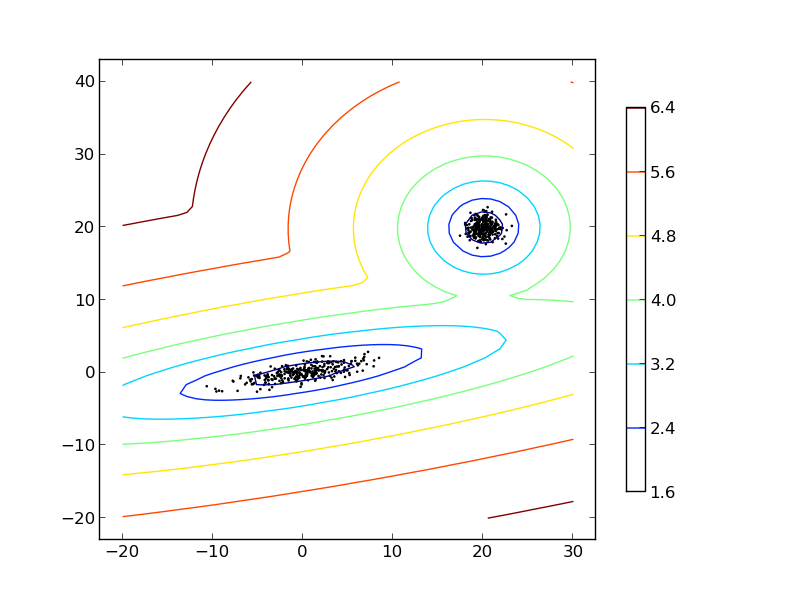
\includegraphics[width=\textwidth]{gmm_original.png}
                    \caption{Original figure, 2 components}
                    \label{fig:orig}
            \end{subfigure}%
            ~ %add desired spacing between images, e. g. ~, \quad, \qquad etc.
              %(or a blank line to force the subfigure onto a new line)
            \begin{subfigure}[h]{0.3\textwidth}
                    \centering
                    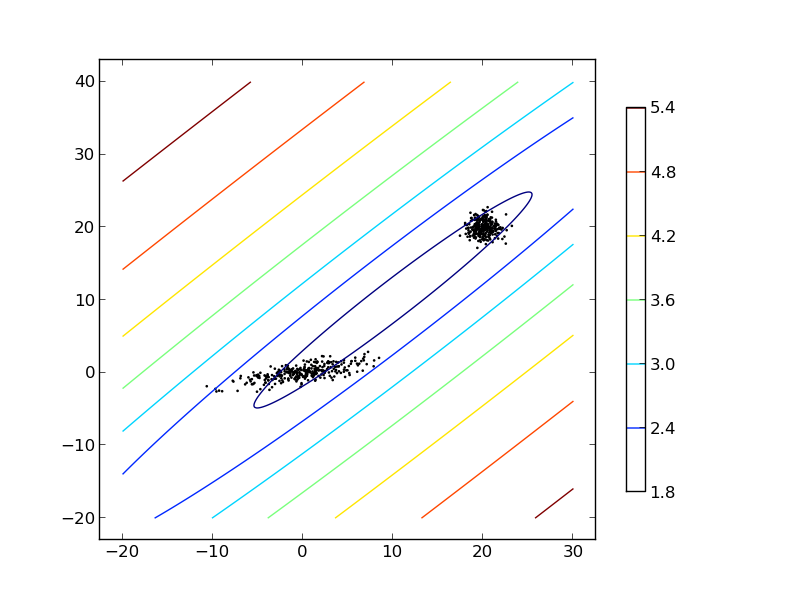
\includegraphics[width=\textwidth]{gmm_comp1.png}
                    \caption{only 1 component}
                    \label{fig:comp1}
            \end{subfigure}
            ~ %add desired spacing between images, e. g. ~, \quad, \qquad etc.
              %(or a blank line to force the subfigure onto a new line)
            \begin{subfigure}[h]{0.3\textwidth}
                    \centering
                    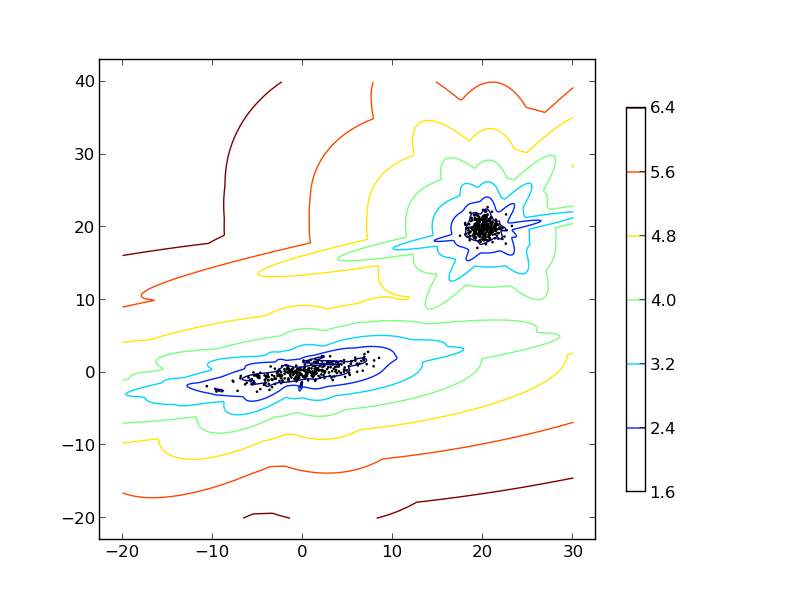
\includegraphics[width=\textwidth]{gmm_comp30.png}
                    \caption{30 components for fun}
                    \label{fig:comp30}
            \end{subfigure}
            \caption{Density estimation for a mixture of Gaussians (2, 1, 30 components)}\label{fig:GMMex}
    \end{figure}

    \begin{figure}
            \centering
            \begin{subfigure}[h]{0.5\textwidth}
                    \centering
                    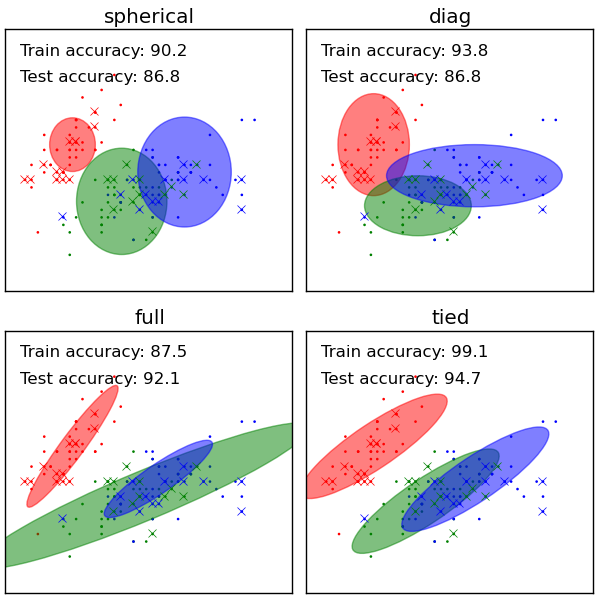
\includegraphics[width=\textwidth]{gmm_class_orig.png}
                    \caption{GMM classification, partially supervised}
                    \label{fig:GMM_orig}
            \end{subfigure}%
            ~ %add desired spacing between images, e. g. ~, \quad, \qquad etc.
              %(or a blank line to force the subfigure onto a new line)
            \begin{subfigure}[h]{0.5\textwidth}
                    \centering
                    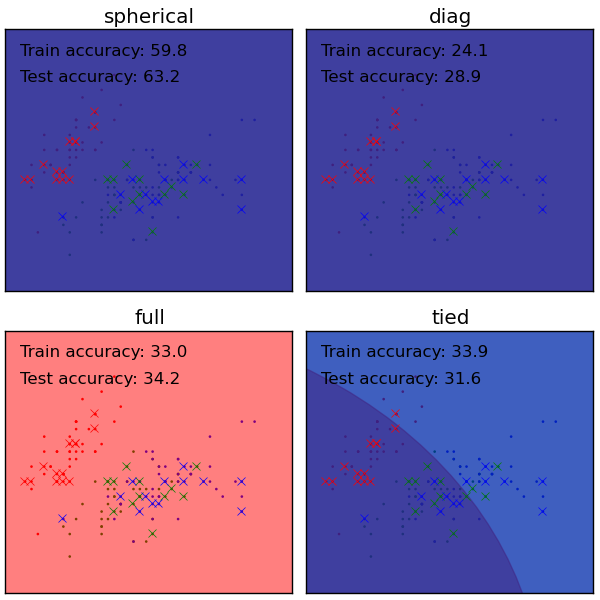
\includegraphics[width=\textwidth]{gmm_class_DPfail.png}
                    \caption{DPGMM attempt (failed)}
                    \label{fig:GMMfail}
            \end{subfigure}
            ~ %add desired spacing between images, e. g. ~, \quad, \qquad etc.
              %(or a blank line to force the subfigure onto a new line)
            \caption{Partially-supervised GMM of iris test data and failed attempt at using Dirichlet Process (DP) GMM on the iris data.  This may make sense, since iris data are so overlapped?}\label{fig:GMM}
    \end{figure}

    \begin{figure}
            \centering
            \begin{subfigure}[h]{0.5\textwidth}
                    \centering
                    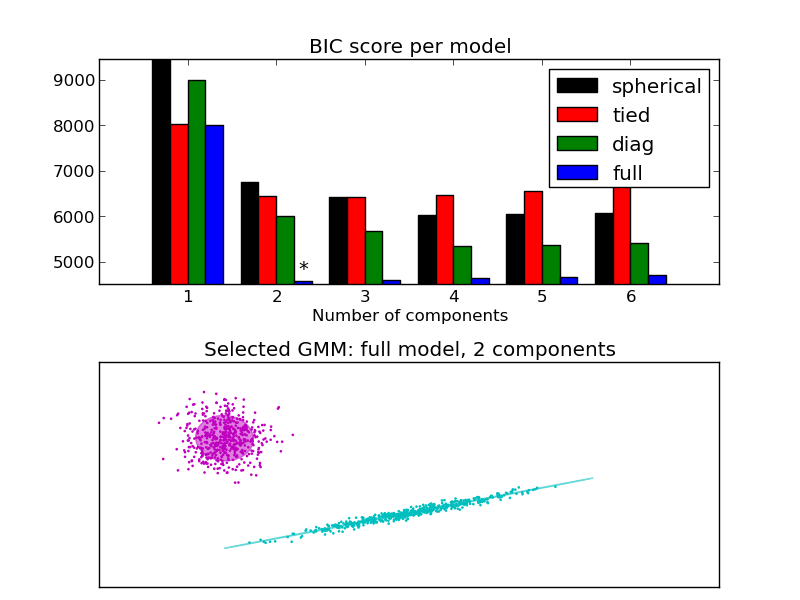
\includegraphics[width=\textwidth]{gmm_select_orig.png}
                    \caption{Selecting GMM model with BIC. 600 data points, seed=0}
                    \label{fig:GMMSelectOrig}
            \end{subfigure}%
            ~ %add desired spacing between images, e. g. ~, \quad, \qquad etc.
              %(or a blank line to force the subfigure onto a new line)
            \begin{subfigure}[h]{0.5\textwidth}
                    \centering
                    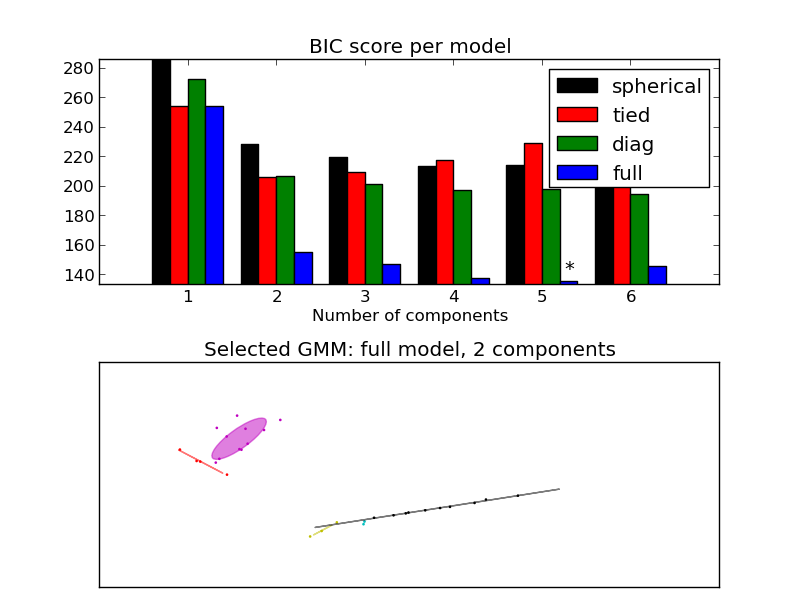
\includegraphics[width=\textwidth]{gmm_select_aic_noseed_n15.png}
                    \caption{Selecting GMM model with AIC. 15 data points, no random seed}
                    \label{fig:GMMSelect15}
            \end{subfigure}
            ~ %add desired spacing between images, e. g. ~, \quad, \qquad etc.
              %(or a blank line to force the subfigure onto a new line)
            \caption{Selecting number of components for GMM with BIC or AIC. Data are randomly generated from two Guassian distributions.}\label{fig:GMMSelect}
    \end{figure}
\end{document}
